% \chapter[基于跨模态语义嵌入的小样本HRRP元学习识别方法]{基于跨模态语义嵌入的小样本HRRP元学习识别方法}
\chapter[基于跨模态语义嵌入的小样本HRRP元学习识别方法]{基于跨模态语义嵌入的小样本HRRP元学习\protect\\ 识别方法}
\label{chap:semantic_fusion}

\section{引言}
\label{sec:semantic_intro}

在前述章节中,本文针对小样本HRRP RATR中的噪声鲁棒性和角度敏感性问题进行了探讨,并提出了基于元学习的解决方案。然而,当可用标注样本极度稀疏(例如单样本或极少样本)且信号质量受限时,仅依赖从一维雷达信号中提取的物理特征,其判别能力往往达到瓶颈,尤其难以区分结构相似、散射特性接近的目标。这种由数据稀疏性引发的特征判别力不足,是制约小样本RATR性能进一步提升的又一关键障碍。因此,探索如何引入独立于物理观测的先验知识来增强模型的区分能力,成为提升小样本识别性能的重要途径。

目标的语义信息,即关于目标类别的高层抽象知识,为此提供了有前景的方向。语义能够提供独立于底层物理特征的判别线索,尤其在物理特征模糊或相似时具有潜力。然而,将文本形式的语义信息与一维HRRP信号有效融合,尤其在小样本框架下,面临显著的模态鸿沟挑战。直接应用视觉领域的跨模态方法或从零学习HRRP到语义的映射均不适用于数据稀疏的场景。近年来,大规模预训练视觉语言模型(Visual Language Model,VLM)如CLIP及其衍生模型RemoteCLIP,通过在海量图文数据上进行训练,学习到了强大的、对齐的视觉与文本语义表示,蕴含了丰富的世界知识和泛化能力,为跨模态知识迁移提供了新的机遇。

本章聚焦于小样本HRRP识别中特征判别性不足与语义信息利用匮乏的问题。本文提出一种名为SHARP的协同跨模态适配方法。该方法的核心在于设计一个轻量级的可学习输入端适配器,将一维HRRP信号“重塑”为二维伪图像,使得本文能够直接利用预训练VLM中强大的、冻结的视觉编码器进行特征提取,从而跨越模态鸿沟。为避免“语义偏见”问题,SHARP采用了一种协同训练策略,在训练适配器时,同时结合了跨模态对齐损失与视觉特定对比损失。前者保证了特征的语义相关性,后者则直接在VLM提取的视觉特征空间内强制执行类内紧凑和类间分离,促使适配器学习生成能够保留并强化HRRP信号固有区分性结构的伪图像。通过这种协同优化,本文旨在使VLM提取的特征既包含高级语义信息,又富含对HRRP识别任务至关重要的视觉判别线索。在小样本识别阶段,本文利用这些增强的视觉特征构建类别原型,并可通过语义融合模块进一步精炼原型,最终完成分类。该方法旨在以最小的训练开销有效迁移VLM知识,克服小样本限制。

本章的内容安排如下:第~\ref{sec:semantic_method}~节首先对小样本设定下仅基于物理特征识别的局限性进行分析,然后详细阐述所提出的跨模态语义嵌入的小样本HRRP元学习识别方法,包括电磁语义进化方法、协同适配器训练机制、语义精炼策略以及整体算法流程;第~\ref{sec:experiments_semantic}~节基于仿真实验结果和实测数据硬件平台测试结果,对所提方法的性能进行验证和分析;第~\ref{sec:semantic_summary}~节对本章的研究工作进行总结。

\section{融合跨模态语义嵌入的元学习识别方法}
\label{sec:semantic_method}

本节详细介绍本文提出的融合跨模态语义嵌入的小样本HRRP识别方法SHARP。首先分析小样本HRRP特征判别性不足的挑战以及引入语义信息的动机。然后,介绍雷达目标语义信息的定义与表示方法。接着,重点阐述如何通过适配器和预训练VLM实现HRRP特征的跨模态提取与语义对齐。之后,讨论基于语义增强特征的小样本识别策略。最后给出整体框架和算法流程。

\subsection{小样本HRRP特征判别性挑战与语义引入}
\label{subsec:semantic_challenge}

在小样本设定下,每个目标类别仅提供极少数标注样本(例如 $K=1$ 或 $K=5$)。对于 HRRP 信号而言,其形态对目标的姿态角、噪声水平以及雷达参数等观测条件高度敏感。因此,这有限的 $K$ 个样本往往形态各异,难以充分表征类别的内在不变特性。若仅依赖这些稀疏样本训练深度模型 $f_\Theta$ 来提取物理特征 $\phi_\theta(\mathbf{x})$,所学特征的判别能力将面临严峻挑战。一方面,不同类别但物理结构相似的目标如飞机的不同改型,在某些观测角度下产生极其相似的 HRRP,导致特征空间中的混淆。另一方面,当信噪比较低或存在强干扰时,HRRP 信号本身的结构信息可能退化,进一步削弱了基于物理特征的区分度。

在这种情况下,单纯依赖可能存在模糊性或相似性的物理特征 $\phi_\theta(\mathbf{x})$ 进行分类,其性能将受到根本性制约。引入独立于物理观测条件的语义信息 $s$ 提供了一条克服此局限的途径。语义信息 $s$ 承载了关于目标类别的高层抽象知识,如其功能属性如战斗机、运输机、关键结构特征如单引擎、三角翼、制造商等。即使两个类别 $c_1$ 和 $c_2$ 的 HRRP 样本 $\mathbf{x}_1, \mathbf{x}_2$ 在物理特征空间中距离相近,它们的语义描述 $s_{c_1}, s_{c_2}$ 通常具有显著差异。若能在分类决策中有效融合物理特征与语义信息,则有望显著提升在挑战性条件下的识别准确性与鲁棒性。

视觉 FSL 的研究\upcite{zhang_simple_2024, chen_improving_2022}已证实了语义增强的有效性。然而,将文本语义与一维 HRRP 信号直接融合存在显著的模态差异。在小样本条件下从头学习跨模态映射是不可行的。幸运的是,大规模 VLM 如 RemoteCLIP\upcite{liu_remoteclip_2024} 通过在海量图文对上的预训练,已学习到强大的、对齐的视觉与语义表示能力。这启发本文思考:是否可以不直接融合 HRRP 和文本,而是将 HRRP 信号适配给 VLM 的视觉通路,利用 VLM 内部已经存在的视觉-语义对齐关系。从这个思路出发,本文提出通过一个输入端适配器将 HRRP 转换为 VLM 视觉编码器 $f_V$ 可处理的伪图像。然而,仅仅强制 $f_V$ 输出的视觉特征 $\mathbf{z}_V$ 与文本特征 $\mathbf{z}_T$ 对齐,可能导致 VLM 忽略对 HRRP 分类至关重要的、但难以语言化的结构细节,即产生“语义偏见”。因此,本文的方法SHARP不仅要实现这种跨模态适配与对齐,还要通过特定的训练策略来确保提取的特征 $\mathbf{z}_V$ 保留 HRRP 固有的判别信息,从而为小样本识别奠定坚实基础。

\subsection{雷达目标语义信息的定义与表示}
\label{subsec:semantic_representation}

为了利用语义信息,首先需要为每个目标类别 $c$ 定义并获取其语义表示 $\mathbf{z}_{T,c}$。这里的语义信息 $s_c$ 指的是关于类别 $c$ 的文本描述。与简单的类别名称相比,更丰富、更具区分性的文本描述通常能带来更好的效果。

本文采用语义进化(Semantic Evolution)\upcite{zhang_simple_2024}的方法来生成高质量的语义描述 $s_c$。该过程通常包括两个步骤:首先,为每个类别名称 $c$(例如“F-16”)人工指定一个初始的、简短的定义或描述,也可通过查表方式获得。然后,利用大型语言模型(Large Language Model,LLM)对这个初始描述进行扩展和润色,要求LLM生成一段包含该目标类别关键特征如功能、尺寸、典型结构、制造商等的、更详细、更具区分性的文本描述 $s_c$。例如,对于“F-16”,生成的描述可能包含“单引擎多用途战斗机,具有边条翼和气泡式座舱盖,由通用动力公司研制”等信息。为实现语义进化,需要我们设计一段合理的Prompt供大模型输出,经过设计后本文中使用的Prompt为“\textit{Consider the aircraft \{Class Name\}. Briefly expand on \{Piror Definition\} by detailing key radar-significant features relevant for HRRP identification. Maintain scientific accuracy within a single concise paragraph.}” 具体地,一个语义进化过程示例如图~\ref{fig:semevo_framework}~所示。基于LLM生成的语义信息仅描述目标类型,而不生成对其他类型的描述,因此不存在信息泄露的问题,符合FSL的基本范式。

% --- 整体框架图占位符 ---
\begin{figure}[h!] \centering %
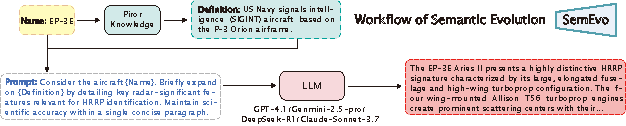
\includegraphics[width=\linewidth]{figures/semevo.pdf}
% 取消注释并替换为你的图表文件
\caption{SemEvo方法流程示意图} \label{fig:semevo_framework} % 更新图表标签
\end{figure}

得到高质量的文本描述 $s_c$ 后,本文利用预训练VLM $\Phi$ 中的冻结文本编码器 $f_T$(参数为 $\theta_T$)将其编码为高维语义特征向量。为了便于后续计算相似度,通常还会进行L2归一化:
\begin{equation}
    \mathbf{z}_{T,c} = \text{normalize}(f_T(s_c; \theta_T)) \in \mathbb{R}^{d_T}
    \label{eq:semantic_encoding}
\end{equation}
其中 $d_T$ 是VLM文本特征的维度。这个过程可以离线完成,为每个类别(包括基类别和新类别)预先计算并存储其语义特征向量 $\mathbf{z}_{T,c}$。这些语义向量 $\mathbf{z}_{T,c}$ 将在后续的适配器训练和小样本分类阶段使用。

\subsection{迁移领域基础模型的HRRP特征提取}
\label{subsec:hrrp_feature_vlm}

为了利用预训练 VLM $\Phi$ 强大的视觉编码器 $f_V$(参数为 $\theta_V$)来处理一维 HRRP 信号,同时克服模态鸿沟和潜在的语义偏见,本文设计了一个输入端适配器 (Input-End Adapter) $h_{1D2D}$(参数为 $\theta_{Ad}$)并为其制定了一个协同训练目标 (Synergistic Training Objective)。

适配器 $h_{1D2D}$ 负责将输入的一维 HRRP 信号 $\mathbf{x}_H \in \mathbb{R}^{L}$,输入通道 $C_{in}=1$,转换为符合 $f_V$ 输入要求的二维伪图像 $\mathbf{x}_{pseudo} \in \mathbb{R}^{C_{out} \times H \times W}$(例如 $C_{out}=3, H=W=224$)。本文采用基于 MLP 的结构实现该适配器:输入 $\mathbf{x}_H$ 首先被展平,然后通过包含非线性激活 ReLU的全连接层进行变换和维度扩展,最终投影到目标维度 $C_{out} \times H \times W$,并通过 Tanh 激活函数约束输出范围,最后重塑为图像格式:
\begin{equation} \mathbf{x}_{pseudo} = h_{1D2D}(\mathbf{x}_H; \theta_{Ad}) = \text{Reshape}(\text{Tanh}(\text{MLP}(\text{Flatten}(\mathbf{x}_H)))). \label{eq:adapter_1d2d} \end{equation}
该适配器是整个方法中主要的需训练模块,VLM 的编码器 $f_V$ 和 $f_T$ 均保持冻结。

适配器的训练在基类数据集 $\mathcal{D}_{\text{base}}$ 上进行,其核心在于协同优化两个互补的损失函数。对于训练批次中的每个样本 $(\mathbf{x}_H, y=c)$,首先通过适配器和冻结的 $f_V$ 提取视觉特征 $\mathbf{z}_V = f_V(h_{1D2D}(\mathbf{x}_H; \theta_{Ad}); \theta_V)$,并进行 L2 归一化得到 $\mathbf{z}_{V, norm} = \text{normalize}(\mathbf{z}_V)$。同时,获取该类别对应的预计算好的归一化语义特征 $\mathbf{z}_{T,c}$。

% --- 整体框架图占位符 ---
\begin{figure}[h!] \centering %
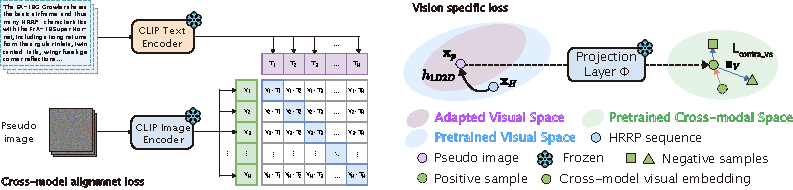
\includegraphics[width=\linewidth]{align_loss.pdf}
% 取消注释并替换为你的图表文件
% \fbox{图 5.1: SHARP整体框架示意图 (占位符)} % 更新图号
\caption{各损失函数计算方法示意图:(a) 多模态对齐损失 (b) 视觉特定对比损失} \label{fig:align} % 更新图表标签
\end{figure}

第一个损失是跨模态对齐损失 $L_{align}$,它旨在确保适配器生成的伪图像能够被 $f_V$ 解读为与目标语义一致的特征。如图~\ref{fig:align}~所示,跨模态对齐损失通过最大化批次内匹配的图像-文本对特征之间的余弦相似度,同时最小化不匹配对的相似度来实现。本文采用基于余弦相似度的损失: \begin{equation} L_{align}(\theta_{Ad}) = 1 - \mathbb{E}_{(\mathbf{x}_H, y=c) \sim \mathcal{D}_{\text{base}}} \left[ \cos(\mathbf{z}_{V, norm}, \mathbf{z}_{T,c}) \right], \label{eq:adapter_align_loss_detail} \end{equation} 其中 $\cos(\mathbf{a}, \mathbf{b}) = \mathbf{a}^T \mathbf{b}$ 。该损失将 VLM 的高级语义知识迁移到适配器的学习中。

然而,仅依赖 $L_{align}$ 可能导致 $\mathbf{z}_V$ 过于关注与文本描述强相关的特征,而忽略 HRRP 信号中独特的、难以语言化的结构信息。为了缓解这种“语义偏见”并增强特征对 HRRP 任务的特定判别力,本文引入第二个损失:视觉特定对比损失 $L_{cl\_v2v}$。该损失直接在 VLM 提取的视觉特征空间 $\mathbf{z}_V$ 中操作,采用监督对比学习(Supervised Contrastive Learning)的形式。如图~\ref{fig:align}~所示,在同一个训练批次内,对于一个锚点特征 $\mathbf{z}_{V,i}$,对应标签 $y_i$,来自同一类别的其他样本特征 $\mathbf{z}_{V,k}$ ($y_k=y_i, k \neq i$) 被视为正样本,而来自不同类别的样本特征 $\mathbf{z}_{V,j}$ ($y_j \neq y_i$) 被视为负样本。InfoNCE 损失函数被用来拉近同类样本特征,推远不同类样本特征:
\begin{equation} L_{cl\_v2v}(\theta_{Ad}) = -\frac{1}{|\mathcal{B}|}\sum_{i \in \mathcal{B}} \log \frac{\sum_{k \in \mathcal{P}(i)} \exp(\text{sim}(\mathbf{z}_{V,i}, \mathbf{z}_{V,k}) / \tau_v)}{\sum_{a \in \mathcal{A}(i)} \exp(\text{sim}(\mathbf{z}_{V,i}, \mathbf{z}_{V,a}) / \tau_v)}, \label{eq:adapter_contrastive_loss} \end{equation}
其中 $\mathcal{B}$ 是批次索引集,$\mathcal{P}(i)$ 是锚点 $i$ 的正样本索引集,$\mathcal{A}(i)$ 是除 $i$ 之外的所有样本索引集,$\text{sim}(\cdot, \cdot)$ 为余弦相似度,$\tau_v$ 是视觉对比损失的温度超参数。

最终,适配器的协同训练目标是最小化这两个损失的加权和: \begin{equation} L_{total}(\theta_{Ad}) = L_{align}(\theta_{Ad}) + \lambda_{v2v} L_{cl\_v2v}(\theta_{Ad}), \label{eq:adapter_total_loss} \end{equation} 其中 $\lambda_{v2v}$ 是平衡两个损失项贡献的超参数。通过这种协同优化,适配器 $h_{1D2D}$ 被引导学习生成一种特殊的伪图像表示,使得冻结的 VLM 视觉编码器 $f_V$ 提取的特征 $\mathbf{z}_V$ 既能在宏观上与语义 $\mathbf{z}_T$ 对齐,又能在微观结构上保持对 HRRP 信号内在差异的敏感性,从而获得更适合小样本 HRRP 识别任务的高质量特征。训练完成后,对于任何 HRRP 输入 $\mathbf{x}_H$,组合 $h_{1D2D}(\cdot; \theta_{Ad})$ 和 $f_V(\cdot; \theta_V)$ 即可提取其增强的、归一化的视觉特征 $\mathbf{z}_V$。

\subsection{基于语义增强特征的元学习策略}
\label{subsec:semantic_fsl_strategy}

在获得经过协同训练增强的视觉特征 $\mathbf{z}_V$ 后,本文在元测试阶段采用基于原型网络(ProtoNet)\upcite{tian_open_2022} 的度量学习策略来执行 $N$-way $K$-shot 分类任务。在此阶段,适配器 $h_{1D2D}$、VLM 编码器 $f_V, f_T$ 以及后续引入的 SemAlign 模块 $h_F$ 均保持冻结状态。

对于从新类集合 $\mathcal{D}_{\text{novel}}$ 中采样的一个任务,包含支持集 $\mathcal{S} = \{(\mathbf{x}_{H,i}, y_i)\}_{i=1}^{N \times K}$ 和查询集 $\mathcal{Q} = \{\mathbf{x}_{H,q}\}$。首先,本文为支持集中的每个样本 $\mathbf{x}_{H,i}$ 通过组合 $h_{1D2D}$ 和 $f_V$ 提取其归一化的视觉特征 $\mathbf{z}_{V,i} = \text{normalize}(f_V(h_{1D2D}(\mathbf{x}_{H,i})))$。

然后,本文计算每个类别 $c \in \{1, \dots, N\}$ 的基础视觉原型 (Visual Prototype) $\mathbf{u}_c$,即该类别 $K$ 个支持样本视觉特征的算术平均值:
\begin{equation} \mathbf{u}_c = \frac{1}{K} \sum_{\{(\mathbf{x}_{H,i}, y_i=c) \in \mathcal{S}\}} \mathbf{z}_{V,i}. \label{eq:visual_prototype} \end{equation}
$\mathbf{u}_c$ 代表了类别 $c$ 在 VLM 视觉特征空间中的经验中心。

尽管 $\mathbf{z}_V$ 已通过协同训练得到增强,但基于 K 个样本计算的 $\mathbf{u}_c$ 仍可能存在偏差,尤其当 K 值极小时,该原型可能无法稳定地代表类别中心。为了进一步提升原型的鲁棒性并利用语义信息进行校准,本文引入了第二阶段的语义利用机制:语义精炼 (Semantic Refinement)。本文采用一个预训练好的 SemAlign 模块 $h_F$(参数为 $\theta_F$),该模块学习根据样本归一化前的视觉特征 $\mathbf{z}'_{V,i} = f_V(h_{1D2D}(\mathbf{x}_{H,i}))$ 和其类别语义特征 $\mathbf{z}_{T,c}$ 来重建一个理想化的视觉表示。

SemAlign 模块的训练目标是在基类数据集 $\mathcal{D}_{\text{base}}$ 上完成的,旨在学习一个从“有噪声”或“个体化”的视觉特征 $\mathbf{z}'_V$ 和类别语义 $\mathbf{z}_T$ 到该类别稳定视觉中心表示的映射。 具体而言,其训练过程旨在最小化模块输出 $\hat{\mathbf{z}}_{V,i} = h_F([\mathbf{z}'_{V,i}; \mathbf{z}_{T,c}]; \theta_F)$ 与该类别 $c$ 在基类数据上预先计算得到的平均视觉中心 $\mathbf{u}_c^{base}$ 之间的距离。本文采用 L1 损失作为重构误差度量,因此 SemAlign 模块的优化目标是:
\begin{equation}
    \theta_F^* = \arg\min_{\theta_F} \mathbb{E}_{(\mathbf{x}_H, y=c) \sim \mathcal{D}_{\text{base}}} \left[ || h_F([\mathbf{z}'_{V,i}; \mathbf{z}_{T,c}]; \theta_F) - \mathbf{u}_c^{base} ||_1 \right]
    \label{eq:semalign_loss_detail}
\end{equation}
其中 $\mathbf{z}'_{V,i} = f_V(h_{1D2D}(\mathbf{x}_{H,i}; \theta_{Ad}^*))$ 是使用已训练好的适配器 $\theta_{Ad}^*$ 提取的归一化前特征。通过最小化这个重构损失,SemAlign 模块 $h_F$ 被训练成一个“去噪器”或“校准器”,它利用类别语义信息 $\mathbf{z}_{T,c}$ 来指导如何从可能存在个体差异或噪声的 $\mathbf{z}'_V$ 中恢复出更接近类别真实中心的表示。

需要明确的是,上式中的目标视觉中心 $\mathbf{u}_c^{base}$ 是在适配器 $h_{1D2D}$ 训练完成之后,离线计算得到的。 对于基类数据集 $\mathcal{D}_{\text{base}}$ 中的每一个类别 $c \in C_{base}$,我们首先使用训练好的适配器 $\theta_{Ad}^*$ 和冻结的视觉编码器 $f_V$ 提取该类别下所有样本 $\{\mathbf{x}_{H,j} | y_j=c\}$ 的归一化前视觉特征 $\{\mathbf{z}'_{V,j}\}$。然后,计算这些特征的算术平均值,得到类别 $c$ 的基类视觉中心:
\begin{equation}
    \mathbf{u}_c^{base} = \frac{1}{|\{j | y_j=c\}|} \sum_{\{j | y_j=c\}} f_V(h_{1D2D}(\mathbf{x}_{H,j}; \theta_{Ad}^*); \theta_V)
    \label{eq:base_class_center}
\end{equation}
这个 $\mathbf{u}_c^{base}$ 代表了在基类充足数据下,类别 $c$ 在 VLM 视觉特征空间中的稳定位置。SemAlign 模块的学习目标就是利用语义信息,将任意输入样本的视觉特征“拉向”其对应类别的这个稳定中心。

在推理时,本文利用冻结的 $h_F$ 为支持集样本生成重建特征 $\hat{\mathbf{z}}_{V,i}$,然后计算平均重建原型 (Mean Reconstructed Prototype) $\mathbf{r}_c$,即对重建特征进行平均并归一化:
\begin{equation} \mathbf{r}_c = \text{normalize} \left( \frac{1}{K} \sum_{\{(\mathbf{x}_{H,i}, y_i=c) \in \mathcal{S}\}} h_F([\mathbf{z}'_{V,i}; \mathbf{z}_{T,c}]; \theta_F^*) \right). \label{eq:reconstructed_prototype} \end{equation}
$\mathbf{r}_c$ 可以视为一个经过语义信息校准的类别中心表示。

最终的类别原型$p_c$ 通过超参数 $\kappa \in [0, 1]$ 对基础视觉原型 $\mathbf{u}_c$ 和平均重建原型 $\mathbf{r}_c$ 进行凸组合得到:
\begin{equation} p_c = (1 - \kappa) \mathbf{u}_c + \kappa \mathbf{r}_c. \label{eq:semantic_fusion_prototype} \end{equation}
$\kappa$ 控制了语义精炼的程度。当 $\kappa=0$ 时,仅使用基础视觉原型;当 $\kappa>0$ 时,融合了语义校准的信息。实验发现(见~\ref{sec:experiments_semantic}~节),$\kappa$ 的最优取值与样本数量 $K$ 相关,在1-shot等极少样本时,适度融合语义信息(如 $\kappa=0.3 \sim 0.5$)效果较好;当样本量稍多(如5-shot及以上)时,基础视觉原型 $\mathbf{u}_c$ 可能已足够可靠,此时 $\kappa=0$ 反而更优。最后,对于查询样本 $\mathbf{x}_{H,q}$,提取其归一化视觉特征 $\mathbf{z}_{V,q} = \text{normalize}(f_V(h_{1D2D}(\mathbf{x}_{H,q})))$。通过计算 $\mathbf{z}_{V,q}$ 与所有 $N$ 个类别原型 $p_c$ 之间的余弦相似度,并应用 Softmax 函数,得到其属于每个类别的概率:
\begin{equation} P(y_q = c | \mathbf{x}_{H,q}) = \frac{\exp(\text{sim}(\mathbf{z}_{V,q}, p_c) / \tau)}{\sum_{j=1}^{N} \exp(\text{sim}(\mathbf{z}_{V,q}, p_j) / \tau)}, \label{eq:classification_semantic} \end{equation}
其中 $\text{sim}(\cdot, \cdot)$ 表示余弦相似度,$\tau$ 是温度超参数。预测标签 $\hat{y}_q$ 被赋予具有最高概率的类别。该策略通过多阶段利用 VLM 的视觉和语义能力,旨在为小样本 HRRP 识别构建更具判别力和泛化性的分类器。

\subsection{整体识别框架与算法流程} \label{subsec:overall_framework_semantic} 所提出的SHARP方法的整体架构与执行流程如图~\ref{fig:sharp_framework}~所示。在预训练阶段,需要使用VLM的文本和视觉编码器同时进行推理,而当适配器训练完成,即可仅依赖适配器和视觉编码器进行测试。SHARP的重要优势在于其利用VLM能力的同时,无需对VLM进行微调,而是仅需对一个简单的MLP$h_{1D2D}$进行训练。该方法整合了离线的语义特征预计算、基于基类数据的模型训练(包括适配器和 SemAlign 模块)以及面向新类的小样本识别即元测试三个主要阶段。

% --- 整体框架图占位符 ---
\begin{figure}[h!] \centering %
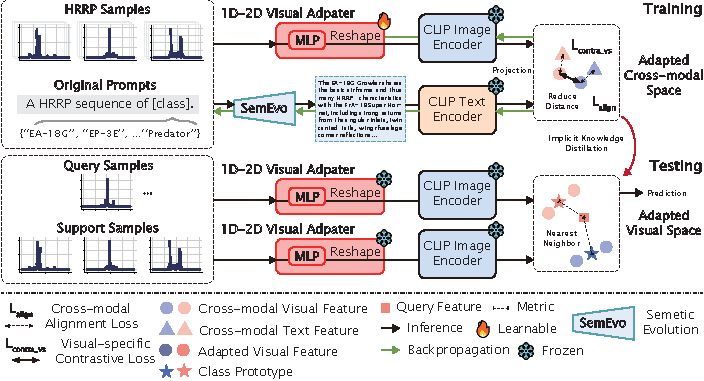
\includegraphics[width=\linewidth]{method3.pdf}
% 取消注释并替换为你的图表文件
% \fbox{图 5.1: SHARP整体框架示意图 (占位符)} % 更新图号
\caption{SHARP方法整体流程示意图} \label{fig:sharp_framework} % 更新图表标签
\end{figure}

具体的算法流程分为三个部分。

i. 首先,适配器协同训练过程详见算法~\ref{alg:adapter_training_synergistic}。该算法在基类数据集上迭代,通过最小化结合了跨模态对齐损失 $L_{align}$ 和视觉特定对比损失 $L_{cl\_v2v}$ 的协同目标函数 $L_{total}$,来优化适配器 $h_{1D2D}$ 的参数 $\theta_{Ad}$,而 VLM 参数保持冻结。

ii. 其次,SemAlign 模块训练过程在算法~\ref{alg:semalign_training}~中描述。此阶段同样在基类数据集上进行,但此时适配器 $\theta_{Ad}^*$ 和 VLM $f_V$ 均已冻结。SemAlign 模块 $h_F$(参数 $\theta_F$)以基类样本归一化前的视觉特征 $\mathbf{z}'_V$和语义特征 $\mathbf{z}_T$ 作为输入,其训练目标是最小化其输出与预先计算好的基类平均视觉中心 $\mathbf{u}_c^{base}$ 之间的重建误差 $L_{recon}$。

iii. 最后,元测试流程展示于算法~\ref{alg:fsl_testing_sharp}。对于一个来自新类的数据集 $\mathcal{D}_{\text{novel}}$ 的 $N$-way $K$-shot 任务,算法首先使用训练好的适配器 $\theta_{Ad}^*$ 和冻结的 $f_V$ 提取支持集样本的视觉特征 $\mathbf{z}_V$。然后计算每个类别的基础视觉原型 $\mathbf{u}_c$。若融合参数 $\kappa > 0$,则利用预训练好的 SemAlign 模块 $\theta_F^*$ 和语义特征 $\mathbf{z}_T$ 计算重建原型 $\mathbf{r}_c$。最终分类原型 $p_c$ 通过式~(\ref{eq:semantic_fusion_prototype})~进行融合。对于查询样本,提取其特征 $\mathbf{z}_{V,q}$,并根据其与各类别原型 $p_c$ 的余弦相似度,通过 Softmax计算归属概率,从而完成分类预测。

\begin{algorithm}[htbp]
\caption{SHARP 适配器协同训练阶段} \label{alg:adapter_training_synergistic}
\begin{algorithmic}[1]
\REQUIRE 基类数据集 $\mathcal{D}_{\text{base}}$, 冻结的 VLM 视觉编码器 $f_V(\cdot; \theta_V)$ 和文本编码器 $f_T(\cdot; \theta_T)$, 预计算的语义特征 $\{\mathbf{z}_{T,c}\}_{c \in C_{base}}$, 超参数 $\lambda_{v2v}, \tau_v$, 学习率 $\eta_{Ad}$, 训练轮数 $E_{Ad}$
\ENSURE 优化后的适配器参数 $\theta_{Ad}^*$
\STATE 初始化适配器参数 $\theta_{Ad}$
\FOR{轮次 = 1 到 $E_{Ad}$}
    \FOR{每个批次 $\mathcal{B} = \{(\mathbf{x}_{H,i}, y_i=c_i)\}_{i=1}^{B_{size}} \subset \mathcal{D}_{\text{base}}$}
        \STATE 计算原始视觉特征 $\mathbf{z}'_{V,i} = f_V(h_{1D2D}(\mathbf{x}_{H,i}; \theta_{Ad}); \theta_V)$ 对于 $i \in \mathcal{B}$
        \STATE 归一化视觉特征 $\mathbf{z}_{V,i} = \text{normalize}(\mathbf{z}'_{V,i})$ 对于 $i \in \mathcal{B}$
        \STATE 获取文本特征 $\mathbf{z}_{T,c_i}$ 对于 $i \in \mathcal{B}$
        \STATE 计算对齐损失 $L_{align} = 1 - \frac{1}{B_{size}} \sum_{i \in \mathcal{B}} \cos(\mathbf{z}_{V,i}, \mathbf{z}_{T,c_i})$
        \STATE 计算对比损失 $L_{cl\_v2v}(\{\mathbf{z}_{V,i}\}, \{c_i\})$ \% 式~(\ref{eq:adapter_contrastive_loss})
        \STATE 计算总损失 $L_{total} = L_{align} + \lambda_{v2v} L_{cl\_v2v}$
        \STATE 计算梯度 $\nabla_{\theta_{Ad}} L_{total}$
        \STATE 更新参数 $\theta_{Ad} \leftarrow \theta_{Ad} - \eta_{Ad} \nabla_{\theta_{Ad}} L_{total}$ % $\eta_{Ad}$ = 学习率
    \ENDFOR % 结束批次循环
\ENDFOR % 结束轮次循环
\STATE 存储训练好的参数 $\theta_{Ad}^* \leftarrow \theta_{Ad}$
\end{algorithmic}
\end{algorithm}

% ----- Algorithm 5.2: SemAlign Training -----
\begin{algorithm}[htbp]
\caption{SHARP SemAlign 模块训练阶段}
\label{alg:semalign_training}
\begin{algorithmic}[1]
\REQUIRE 基类数据集 $\mathcal{D}_{\text{base}}$, 训练好的适配器 $\theta_{Ad}^*$, 冻结的 $f_V, f_T$, 语义特征 $\{\mathbf{z}_{T,c}\}_{c \in C_{base}}$, 预计算的基类视觉中心 $\{\mathbf{u}_c^{base}\}_{c \in C_{base}}$, 学习率 $\eta_F$, 训练轮数 $E_F$
\ENSURE 优化后的 SemAlign 参数 $\theta_F^*$
\STATE 初始化 SemAlign 参数 $\theta_F$
\FOR{轮次 = 1 到 $E_F$}
    \FOR{每个批次 $\mathcal{B} = \{(\mathbf{x}_{H,i}, y_i=c_i)\}_{i=1}^{B_{size}} \subset \mathcal{D}_{\text{base}}$}
        \STATE 初始化批次损失 $L_{batch} = 0$
        \FOR{$i = 1$ 到 $B_{size}$}
            \STATE 计算原始视觉特征 $\mathbf{z}'_{V,i} = f_V(h_{1D2D}(\mathbf{x}_{H,i}; \theta_{Ad}^*); \theta_V)$ \% 冻结 $\theta_{Ad}^*, \theta_V$
            \STATE 获取文本特征 $\mathbf{z}_{T,c_i}$
            \STATE 重建特征 $\hat{\mathbf{z}}_{V,i} = h_F([\mathbf{z}'_{V,i}; \mathbf{z}_{T,c_i}]; \theta_F)$ \% 输入原始 $\mathbf{z}'_{V,i}$
            \STATE 获取基类中心 $\mathbf{u}_{c_i}^{base}$
            \STATE 计算 L1 损失 $L_{recon, i} = || \hat{\mathbf{z}}_{V,i} - \mathbf{u}_{c_i}^{base} ||_1$
            \STATE 累加损失 $L_{batch} \leftarrow L_{batch} + L_{recon, i}$
        \ENDFOR % 结束内循环
        \STATE 平均批次损失 $L_{avg\_batch} = L_{batch} / B_{size}$
        \STATE 计算梯度 $\nabla_{\theta_F} L_{avg\_batch}$
        \STATE 更新参数 $\theta_F \leftarrow \theta_F - \eta_F \nabla_{\theta_F} L_{avg\_batch}$ % $\eta_F$ = 学习率
    \ENDFOR % 结束批次循环
\ENDFOR % 结束轮次循环
\STATE 存储训练好的参数 $\theta_F^* \leftarrow \theta_F$
\end{algorithmic}
\end{algorithm}

\begin{algorithm}[htbp]
\caption{SHARP 元测试阶段}
\label{alg:fsl_testing_sharp}
\begin{algorithmic}[1]
\REQUIRE 训练好的 $\theta_{Ad}^*, \theta_F^*$, 冻结的 $f_V, f_T$, 语义特征 $\{\mathbf{z}_{T,c}\}_{c \in C_{novel}}$, 新任务 $(\mathcal{S}, \mathcal{Q})$(包含 $N$ 个新类,每类 $K$ 个支持集样本),超参数 $\kappa, \tau$
\ENSURE 查询集 $\mathcal{Q}$ 的预测标签 $Y_{pred}$
\STATE 初始化原型 $P = \{ p_c \}_{c=1}^N$
\FOR{$c = 1$ 到 $N$}
    \STATE 初始化 $\mathbf{u}_c=\mathbf{0}$, $\mathbf{r}_c^{sum}=\mathbf{0}$
    \STATE 获取支持集样本 $\mathcal{S}_c = \{(\mathbf{x}_{H,i}, c) \in \mathcal{S}\}$
    \FOR{$(\mathbf{x}_{H,i}, c) \in \mathcal{S}_c$}
        \STATE $\mathbf{x}_{p,i} = h_{1D2D}(\mathbf{x}_{H,i}; \theta_{Ad}^*)$ \% 生成伪图像
        \STATE $\mathbf{z}'_{V,i} = f_V(\mathbf{x}_{p,i}; \theta_V)$          \% 提取原始视觉特征
        \STATE $\mathbf{z}_{V,i} = \text{normalize}(\mathbf{z}'_{V,i})$           \% 归一化视觉特征
        \STATE $\mathbf{u}_c \leftarrow \mathbf{u}_c + \mathbf{z}_{V,i}$             \% 累加视觉特征
        \IF{$\kappa > 0$}
            \STATE $\hat{\mathbf{z}}_{V,i} = h_F([\mathbf{z}'_{V,i}; \mathbf{z}_{T,c}]; \theta_F^*)$ \% 重建 (输入原始 $\mathbf{z}'_V$)
            \STATE $\mathbf{r}_c^{sum} \leftarrow \mathbf{r}_c^{sum} + \hat{\mathbf{z}}_{V,i}$ \% 累加重建特征
        \ENDIF
    \ENDFOR % 结束支持集样本循环
    \STATE $\mathbf{u}_c \leftarrow \mathbf{u}_c / K$                     \% 平均视觉原型 ($K$=样本数)
    \IF{$\kappa > 0$}
        \STATE $\mathbf{r}_c = \text{normalize}(\mathbf{r}_c^{sum} / K)$       \% 平均并归一化重建原型
    \ELSE
        \STATE $\mathbf{r}_c = \mathbf{u}_c$                           \% 如果 $\kappa=0$ 则虚拟赋值
    \ENDIF
    \STATE $p_c \leftarrow (1 - \kappa) \mathbf{u}_c + \kappa \mathbf{r}_c$   \% 融合原型
\ENDFOR % 结束类别循环
\STATE 初始化预测 $Y_{pred} = [~]$
\FOR{$\mathbf{x}_{H,q} \in \mathcal{Q}$}
    \STATE $\mathbf{x}_{p,q} = h_{1D2D}(\mathbf{x}_{H,q}; \theta_{Ad}^*)$  \% 生成伪图像
    \STATE $\mathbf{z}'_{V,q} = f_V(\mathbf{x}_{p,q}; \theta_V)$           \% 提取原始视觉特征
    \STATE $\mathbf{z}_{V,q} = \text{normalize}(\mathbf{z}'_{V,q})$            \% 归一化视觉特征
\STATE 计算得分 $s_c = \text{Score}(\mathbf{z}_{V,q}, p_c)$ 对于 $c=1..N$ \% 式~(\ref{eq:classification_semantic})~余弦相似度
    \STATE 预测 $\hat{y}_q \leftarrow \arg\max_{c} s_c$
    \STATE 将 $\hat{y}_q$ 添加到 $Y_{pred}$
\ENDFOR % 结束查询集样本循环
\end{algorithmic}
\end{algorithm}

\section{实验设计及结果分析} \label{sec:experiments_semantic} 本节通过一系列实验来系统评估所提出的SHARP方法在小样本 HRRP 识别任务上的性能。实验旨在验证核心假设:通过输入端适配器和协同训练目标利用冻结 VLM 视觉编码器,并结合语义原型精炼,能够有效提升识别精度。

本文采用与前述章节一致的实验设置基础,但特别调整了数据集的划分方式,以更契合本章对语义信息和细粒度识别能力的研究重点。我们仍使用SimHRRP数据集,包含12类飞机目标。为了构建一个更具挑战性、更能体现语义信息价值的场景,我们将数据集划分为7个基类 $\mathcal{D}_{\text{base}}$(包含较多样化的类型,如EA-18G, EP-3E, 全球鹰, 捕食者, 幻影2000, IDF, F-2)和5个新类 $\mathcal{D}_{\text{novel}}$(主要包含结构和功能相对接近的战斗机类型,如F-15, F-16, F-18, F-22, F-35)。 这种划分方式使得新类之间的区分更依赖于细微特征和可能存在的语义差异,更能检验模型在小样本条件下利用语义信息进行精细识别的能力。HRRP 信号预处理(长度 $L=1000$,对数-最大值归一化)以及评估指标(在 $\mathcal{D}_{\text{novel}}$ 上进行 5-way $K$-shot ($K=1, 5$) 任务的平均分类精度及 95\% 置信区间,基于 600 次独立采样)保持不变。本文选择 RemoteCLIP (ViT-B/32)\upcite{liu_remoteclip_2024} 作为 VLM $\Phi$,其视觉编码器 $f_V$ 和文本编码器 $f_T$ 在所有阶段均保持冻结。适配器 $h_{1D2D}$ 采用 MLP 结构,将 HRRP 映射为 $3 \times 224 \times 224$ 的伪图像。语义特征 $\mathbf{z}_{T,c}$ 由 Claude-Sonnet-3.7 生成的高质量描述经冻结 $f_T$ 编码并归一化得到。确保复现性,本文将由各大语言模型(包括消融实验中使用的Gemini-2.5-pro,GPT-4.1,DeepSeek-R1)生成的语义描述包括在附录~\ref{chap:llmsem}~中.

适配器 $h_{1D2D}$ 在 $\mathcal{D}_{\text{base}}$ 上进行训练,优化器为 Adam,学习率 $1 \times 10^{-4}$,训练 100 轮。核心在于采用式~(\ref{eq:adapter_total_loss})~的协同训练目标 $L_{total} = L_{align} + \lambda_{v2v} L_{cl\_v2v}$。其中,$L_{align}$ 基于式~(\ref{eq:adapter_align_loss_detail})~的余弦距离,$L_{cl\_v2v}$ 为式~(\ref{eq:adapter_contrastive_loss})的视觉对比损失。除非特别说明,默认设置 $\lambda_{v2v}=0.5$, $\tau_v=0.1$。SemAlign 模块 $h_F$ 同样在 $\mathcal{D}_{\text{base}}$ 上预训练,使用 Adam 优化器和式~(\ref{eq:semalign_loss_detail})~的L1 重建损失。元测试采用原型网络框架,最终原型 $p_c$ 根据式~(\ref{eq:semantic_fusion_prototype}) 计算(默认 $\kappa=0.5$),分类基于式~(\ref{eq:classification_semantic})~的余弦相似度,温度 $\tau=10.0$。

比较基线包括:直接在 HRRP 上训练的 ProtoNet\upcite{tian_open_2022} 和 MAML\upcite{finn_model-agnostic_2017}(均使用 1D CNN 主干);不使用 VLM 视觉编码器、仅融合 1D CNN 特征与语义的 \textbf{1D CNN + Semantics} 方法;以及本文方法的一个变体 {SHARP ($\kappa=0$)},它使用经过协同训练的适配器提取 $\mathbf{z}_V$ 但在推理时不进行语义融合(即仅使用视觉原型 $\mathbf{u}_c$)。本章的完整方法表示为 {SHARP ($\kappa=0.5$)}。

(1)对比实验

实验的主要结果呈现在表~\ref{tab:main_results_adapter_semantic_filled}~中。SHARP ($\kappa=0.5$) 在 SimHRRP 数据集上的 5-way 1-shot 和 5-way 5-shot 任务中均展现出最优性能。具体而言,在 1-shot 设置下,SHARP ($\kappa=0.5$) 达到了 62.63 $\pm$ 1.56\% 的精度,显著优于 ProtoNet (53.12\%) 和 MAML (55.03\%)。这一结果初步证实了通过适配器利用 VLM 视觉编码器的有效性。与SHARP($\kappa=0$) 的 57.43\% 相比,$\kappa=0.5$ 时约 5.20\% 的性能提升表明,在推理阶段利用 SemAlign 模块进行语义原型精炼是有益的。更值得注意的是SHARP($\kappa=0$) 相对于 1D CNN + Semantics (54.77\%) 的优势(约 2.74\%)。这清晰地表明,仅仅将标准 1D CNN 特征与语义融合,其效果不如通过协同训练的适配器来引导强大的 VLM 视觉编码器提取针对 HRRP 的特征。这突显了 VLM 预训练视觉表征的价值以及本文适配和训练方法的有效性。在 5-shot 设置下,各项指标的相对表现趋势保持一致,SHARP($\kappa=0.5$) 达到 76.25 $\pm$ 1.04\%,进一步巩固了结论。

% --- 主要结果表格 (填充数据) ---
\begin{table}[h!]
\centering
\caption{不同方法在5-way K-shot HRRP 识别任务上的识别准确率对比} \label{tab:main_results_adapter_semantic_filled} %
\resizebox{0.8\linewidth}{!}{%
\begin{tabular}{lccc} \toprule \textbf{Method} & \textbf{Backbone} & \makecell{\textbf{5-way 1-shot}\\\textbf{Acc. (\%)}} & \makecell{\textbf{5-way 5-shot}\\\textbf{Acc. (\%)}} \\ \midrule ProtoNet~\cite{tian_open_2022} & 1D-CNN & 53.12 $\pm$ 0.88 & 67.45 $\pm$ 0.71 \\ MAML~\cite{finn_model-agnostic_2017} & 1D-CNN & 55.03 $\pm$ 0.91 & 69.18 $\pm$ 0.69 \\ \midrule 1D CNN + Semantics & 1D-CNN & 54.77 $\pm$ 0.85 & 62.03 $\pm$ 0.66 \\ \midrule SHARP ($\kappa=0$) & ViT-B/32 & 57.43 $\pm$ 1.87 & 74.79 $\pm$ 1.00 \\ \textbf{SHARP ($\kappa=0.5$)} & ViT-B/32 & \textbf{62.63 $\pm$ 1.56} & \textbf{76.25 $\pm$ 1.04} \\ \bottomrule
\end{tabular} %
} % End resizebox
\end{table}
\captionsetup{skip=5pt}

(2)消融实验

本文进一步通过消融实验深入分析SHARP方法内部件的贡献。

协同训练目标中 $L_{cl\_v2v}$ 的作用: 这是验证本章核心创新的关键实验。本文对比了使用完整协同训练目标($L_{align} + \lambda_{v2v} L_{cl\_v2v}$,设 $\lambda_{v2v}=0.5$)与仅使用对齐损失($L_{align}$,即 $\lambda_{v2v}=0$)训练适配器的效果,均在 $\kappa=0$ 的条件下进行测试。结果显示,仅使用对齐损失时,5-way 1-shot 精度为 66.94 $\pm$ 0.83\%。而加入视觉对比损失后,精度显著提升至 73.85 $\pm$ 0.81\%(即SHARP($\kappa=0$) 的结果)。这 6.91\% 的提升幅度有力地证明了 $L_{cl\_v2v}$ 在引导 VLM 提取更具 HRRP 任务特定判别性的视觉特征、克服语义偏见方面起到了关键作用。

%--- 消融实验表格 2: Kappa 值影响 --- 
\begin{table}[h!] 
\centering 
\caption{不同 $\kappa$ 值对 5-way 1-shot 识别准确率的影响} 
\label{tab:ablation_kappa_value} \resizebox{0.5\linewidth}{!}{%
\begin{tabular}{cc} 
\toprule \textbf{Kappa ($\kappa$)} & \textbf{5-way 1-shot Acc. (\%)} \\ \midrule 0.0 (Visual Only) & 57.43 $\pm$ 1.87 \\ 0.1 & 58.51 $\pm$ 1.82 \\ 0.2 & 60.04 $\pm$ 1.75 \\ 0.3 & 61.52 $\pm$ 1.68 \\ 0.4 & 62.49 $\pm$ 1.60 \\ \textbf{0.5} & \textbf{62.63 $\pm$ 1.56} \\ 0.6 & 60.55 $\pm$ 1.65 \\ 0.7 & 55.08 $\pm$ 1.78 \\ 0.8 & 48.13 $\pm$ 1.85 \\ 0.9 & 41.07 $\pm$ 1.90 \\ 1.0 (Recon Only) & 35.52 $\pm$ 1.93 \\ \bottomrule 
\end{tabular}% 
} % End resizebox 
\end{table} 
\captionsetup{skip=5pt}

语义原型精炼($\kappa$ 值)的影响: 通过在 5-way 1-shot 推理时调整 $\kappa$ 值,本文考察了 SemAlign 模块的作用。当 $\kappa=0$ 时(57.43\%),性能已受益于协同训练的 $\mathbf{z}_V$。随着 $\kappa$ 增大,融合了语义校准信息 $\mathbf{r}_c$,性能逐步提升,在 $\kappa=0.5$ 附近达到峰值 62.63\%。当 $\kappa$ 继续增大至 1 时(仅使用 $\mathbf{r}_c$),性能下降至 35.52\%。这表明,在协同训练获得的高质量 $\mathbf{z}_V$ 基础上,通过 $h_F$ 进行适度的语义精炼能够进一步优化原型,但完全依赖重建特征并非最优。

% --- 消融实验表格 3: 语义源影响 --- 
\begin{table}[h!] 
\centering 
\caption{不同语义源对 SHARP ($\kappa=0.5$) 识别准确率的影响} 
\label{tab:ablation_semantic_source} \resizebox{0.8\linewidth}{!}{%
\begin{tabular}{lccc}
\toprule \textbf{Semantic Source} & \textbf{Backbone} & \makecell{\textbf{5-way 1-shot}\\\textbf{Acc. (\%)}} & \makecell{\textbf{5-way 5-shot}\\\textbf{Acc. (\%)}} \\ \midrule Class Name Only & ViT-B/32 & 61.18 $\pm$ 1.62 & 74.75 $\pm$ 1.10 \\ Deepseek-R1 & ViT-B/32 & 61.61 $\pm$ 1.60 & 75.23 $\pm$ 1.08 \\ GPT-4.1 & ViT-B/32 & 61.84 $\pm$ 1.59 & 75.51 $\pm$ 1.07 \\ Gemini-2.5-pro & ViT-B/32 & 62.05 $\pm$ 1.58 & 75.80 $\pm$ 1.06 \\ \textbf{Claude-Sonnet-3.7} & ViT-B/32 & \textbf{62.63 $\pm$ 1.56} & \textbf{76.25 $\pm$ 1.04} \\ \bottomrule 
\end{tabular}% 
} % End resizebox 
\end{table} 
\captionsetup{skip=5pt}

语义描述质量的影响: 使用高质量描述(Claude-Sonnet-3.7)相比仅使用类名作为语义源(用于 $\mathbf{z}_T$ 生成,影响 $L_{align}$ 和 $h_F$),前者(62.63\%,$\kappa=0.5$)比后者(61.18\%,$\kappa=0.5$)精度高出约 1.45\%,验证了高质量语义对于跨模态对齐和原型精炼的重要性。 同时,相较于Deepseek-R1、GPT-4.1、Gemini-2.5-pro,基于Claude-Sonnet-3.7进行语义进化的效果最优(最高提升1.02\%)。最后,可视化分析提供了直观证据,图~\ref{fig:tsne_adapter_semantic}~使用 t-SNE 可视化了新类样本的 $\mathbf{z}_V$ 特征分布。对比仅使用 $L_{align}$ 训练和使用协同训练目标得到的特征空间,后者展现出明显更优的类内聚合度和类间分离度,直观印证了协同训练策略在提升特征判别性上的优势。

% % --- 伪图像示例图占位符 (保持不变) ---
% \begin{figure}[h!]
% \centering
% % 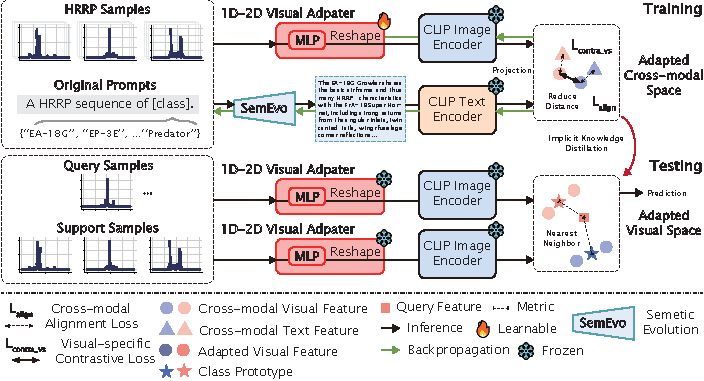
\includegraphics[width=\linewidth]{method3.pdf}
% % \fbox{图 5.2: 适配器生成的伪图像示例 (占位符)}
% \caption{HRRP 信号经适配器转换生成的伪图像示例} \label{fig:pseudo_images_semantic}
% \end{figure}

% --- t-SNE 可视化图占位符 (更新图注) ---
\begin{figure}[h!]
\centering
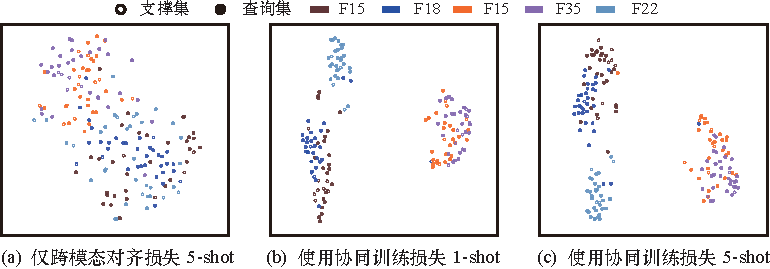
\includegraphics[width=\linewidth]{figures/tsne_pro3.pdf}
% \fbox{图 5.3: 新类别视觉特征 $\mathbf{z}_V$ 的t-SNE可视化 (占位符)}
\caption{不同训练目标下新类别视觉特征的$\mathbf{z}_V$t-SNE 可视化对比} \label{fig:tsne_adapter_semantic} \end{figure}

综合来看,实验结果和可视化分析充分验证了SHARP方法的有效性,特别是协同训练策略在成功适配 VLM 视觉编码器以处理 HRRP 信号、同时保留关键判别信息方面起到的核心作用,以及语义原型精炼带来的进一步性能提升。

(3)硬件部署及实测数据实验

\begin{table}[htbp] % h: here, t: top, b: bottom, p: page of its own
\centering
\caption{树莓派 4B (8GB) 硬件参数}
\label{tab:rpi4b_specs}
\begin{tabular}{l|l} % 使用 | 来模仿示例中的竖线分隔符
\hline
\textbf{设备} & \textbf{具体型号及参数} \\ % 使用 \textbf 模仿示例的加粗表头
\hline
CPU & Broadcom BCM2711, 四核 Cortex-A72 (ARM v8) 64位 SoC \\
\hline
主频 & 1.5GHz (基础频率) \\ % 树莓派4B 基础频率是 1.5GHz 或 1.8GHz,这里用1.5GHz示例
\hline
内存 & 8GB LPDDR4-3200 SDRAM \\
\hline
存储器 & Micro SD 卡插槽 (存储操作系统和数据) \\
\hline
GPU & \makecell[l]{Broadcom VideoCore VI \\ 支持 OpenGL ES 3.1, Vulkan 1.0 \\ H.265 (4Kp60 解码), H.264 (1080p 解码/编码)} \\ % 使用 makecell 实现单元格内换行
\hline
% NPU & 无专用 NPU (可通过 USB 外接加速器) \\ % 明确指出没有NPU
% \hline % 如果上面一行不注释,则保留此hline
NPU & \makecell[l]{无专用 NPU} \\
\hline
% 移除NPU框架支持行,因为没有内置NPU
\end{tabular}
\end{table}

为进一步验证本章提出的 SHARP 方法在接近实际应用环境中的有效性和可行性,我们不仅依赖仿真数据,还开展了基于实测 HRRP 数据和嵌入式硬件平台的实验。考虑到获取和标注大规模、多样化实测 HRRP 数据的固有挑战,以及为了确保研究的聚焦性和深度,本次实测验证战略性地集中于评估 SHARP 方法。选择 SHARP 作为实测验证的核心,主要基于以下考量:首先,SHARP 代表了本研究在应对小样本识别中特征判别力不足这一关键挑战上的最终技术方案,其性能最能体现本研究的整体先进性;其次,该方法创新性地引入了外部 VLM 和语义知识,其实测有效性对于评价这种跨模态知识迁移范式在雷达领域的实际潜力至关重要,这是仿真环境难以完全模拟的;最后,将实验资源集中于对 SHARP 方法的深入实测分析,有助于获取更可靠、更有指导意义的验证结论。我们强调,本论文已在仿真数据上对所有提出的方法及基线进行了全面的比较,此处的实测实验旨在作为关键的补充验证,考察 SHARP 方法在真实数据和资源受限平台上的表现。

本研究的算法验证不仅局限于高性能计算平台,还特别关注了在嵌入式系统上的部署潜力。为此,我们选用了广泛应用的树莓派 4B (Raspberry Pi 4B) 作为代表性的嵌入式开发板进行实验验证。树莓派 4B 以其低成本、高灵活性和丰富的社区支持,成为物联网、边缘计算和快速原型设计的常用平台。其核心板实物和各组分示意如图~\ref{fig:pi}~所示。该开发板的核心是 Broadcom BCM2711 芯片,包含一个四核 ARM Cortex-A72 64位处理器和 VideoCore VI GPU,但关键在于它并未集成专用的神经网络处理单元 (Nueral Processing Unit,NPU)。本实验使用的是配备 8GB LPDDR4 内存的版本,提供了相对宽裕的运行环境,其详细硬件参数已在表~\ref{tab:rpi4b_specs}~中列出。

\begin{figure}[h!]
\centering
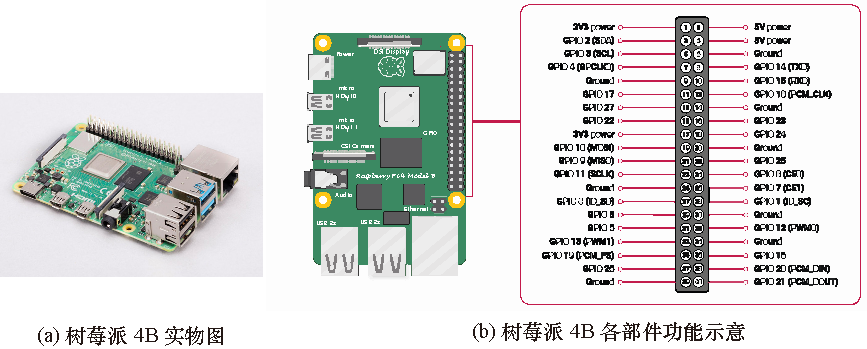
\includegraphics[width=\linewidth]{figures/pi.pdf}
\caption{Raspberry Pi 4B核心板:(a) Raspberry Pi 4B实物 (b) Raspberry Pi 4B各组分示意} 
\label{fig:pi} 
\end{figure}

将在 服务器 端训练完成的 SHARP 模型部署到树莓派 4B 上,需要克服平台差异带来的挑战。我们采用 ONNX (Open Neural Network Exchange) 作为模型转换的中间格式。首先,使用 \texttt{torch.onnx.export()} 函数将训练好的 PyTorch 模型(包括适配器 $h_{1D2D}$ 和 SemAlign 模块 $h_F$,而 VLM 的 $f_V$ 部分由于其标准结构,通常也能较好地转换)导出为 \texttt{.onnx} 文件。这个过程封装了模型的网络结构和权重。随后,在树莓派 4B 上安装针对 ARM 架构的 ONNX Runtime 库。推理过程涉及在树莓派上编写 Python 脚本,利用 ONNX Runtime API 加载 \texttt{.onnx} 模型,对输入的实测 HRRP 数据进行与训练时一致的预处理,然后执行模型推理,最后对输出进行后处理得到分类结果。整个部署流程如图~\ref{fig:4b}~所示的硬件平台实物上执行。由于缺乏 NPU 加速,模型推理完全依赖 CPU,其性能表现是本次实验关注的重点之一。

\begin{figure}[h!]
\centering
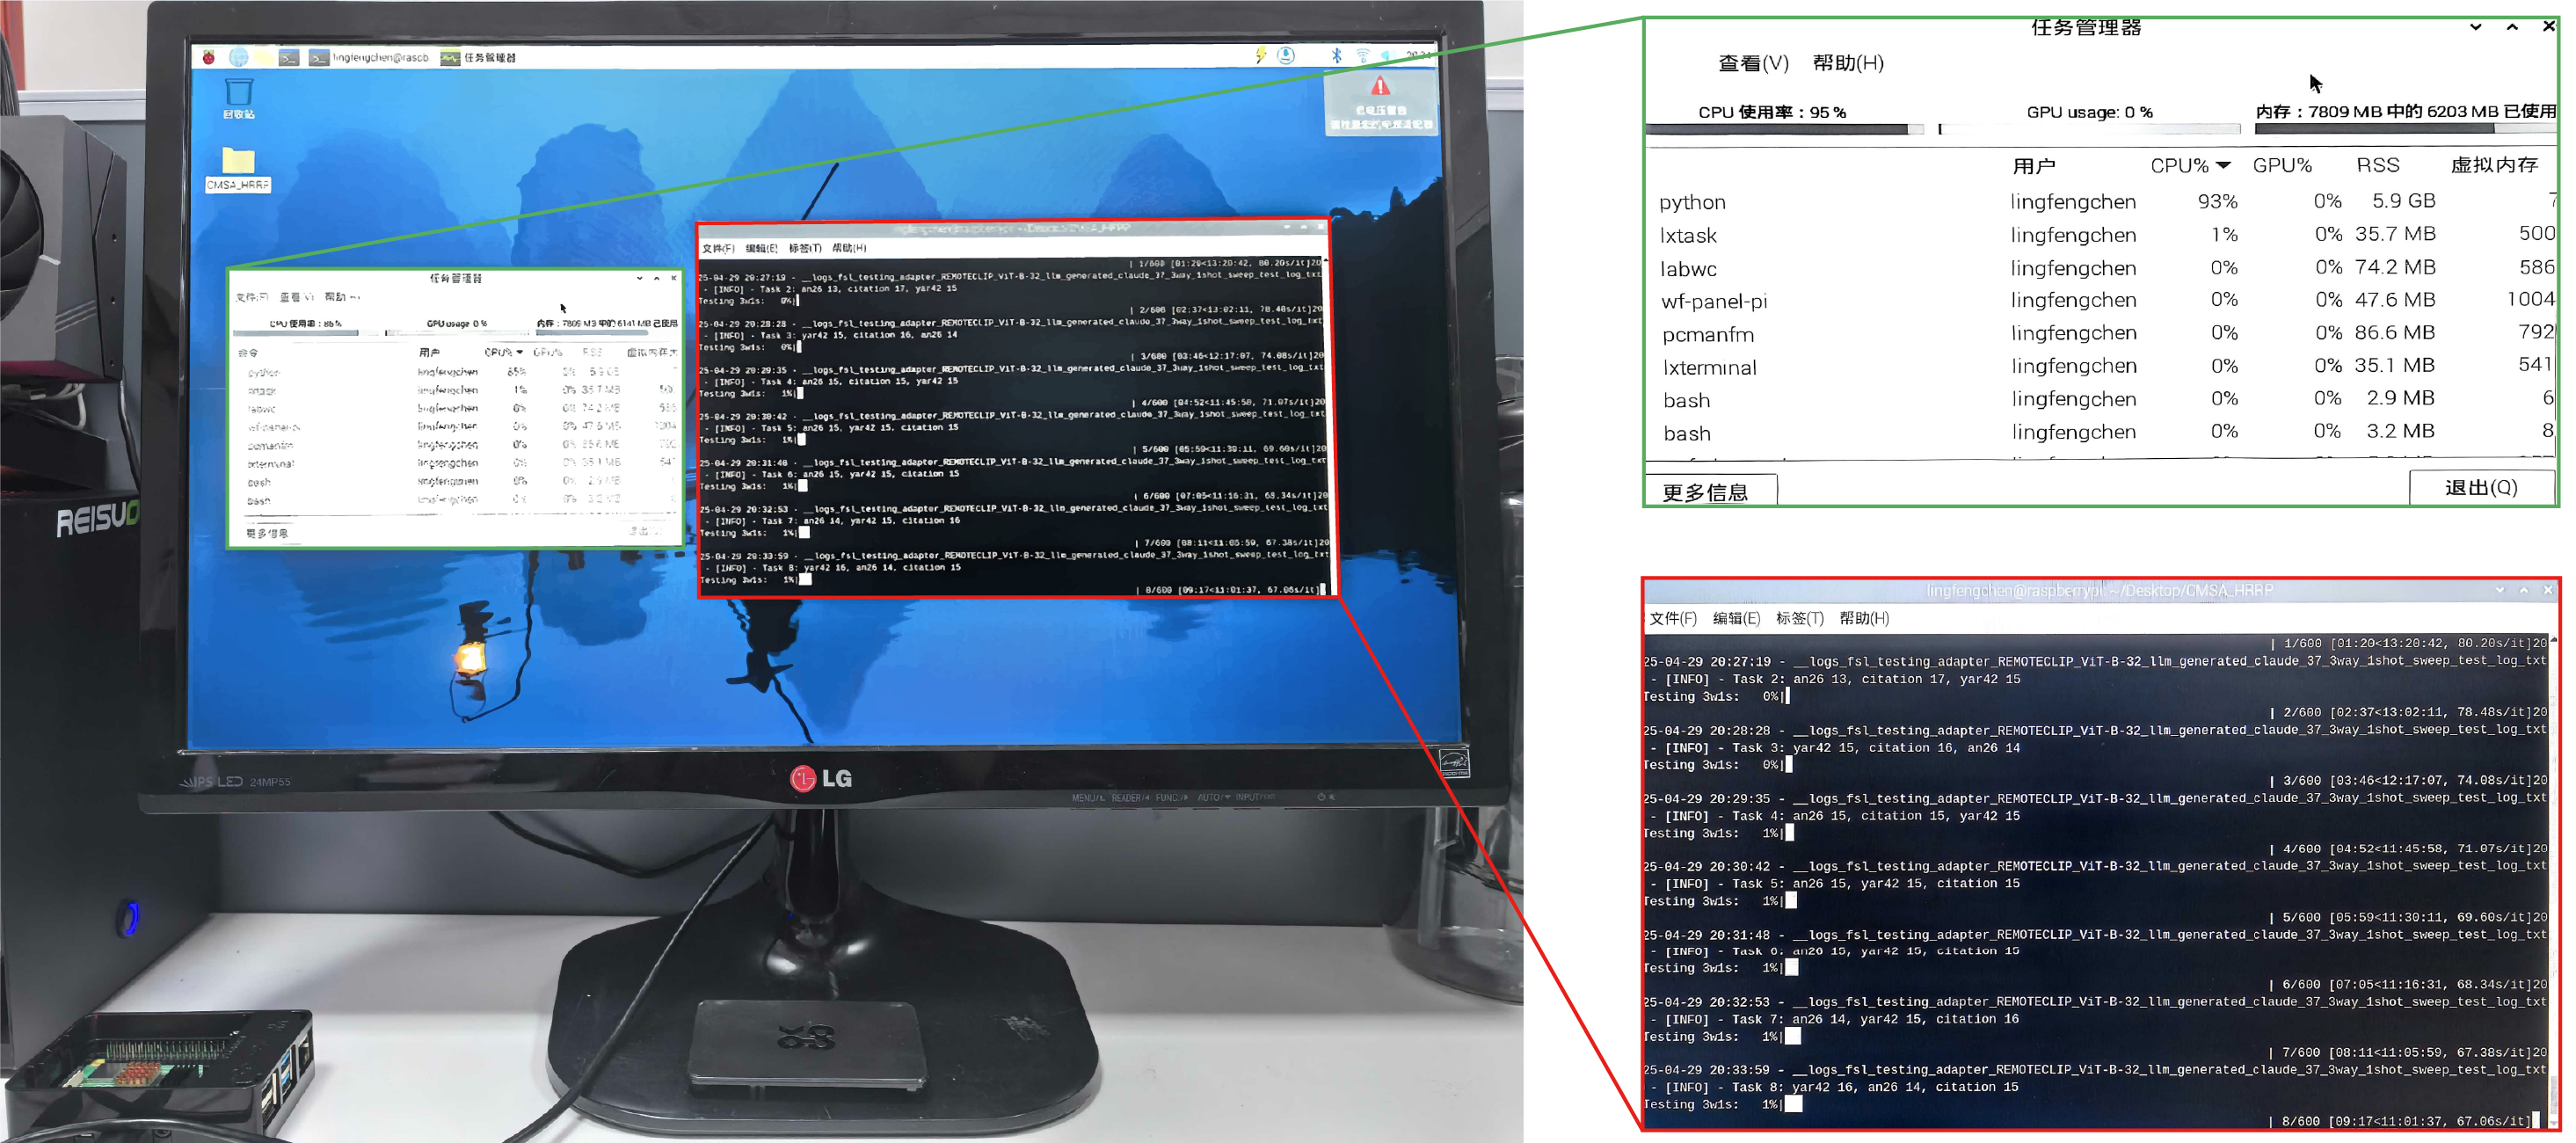
\includegraphics[width=\linewidth]{figures/4b.jpg}
\caption{基于Raspberry Pi 4B的硬件实物平台} 
\label{fig:4b} 
\end{figure}

\begin{table}[h]
\centering
% \resizebox{0.5\linewidth}{!}{%
\caption{三类空天目标实测数据集中各类目标几何参数}
\label{tab:flights_measured}
\begin{tabular}{c c c c}
\toprule
\textbf{目标种类} & \textbf{长度 (m)} & \textbf{翼展 (m)} & \textbf{机高 (m)}\\
\midrule
An-26 & 23.80 & 29.20 & 9.83 \\
% \hline
Yark-42 & 36.38 & 34.88 & 9.83 \\
% \hline
Cessna citation & 14.40 & 15.90 & 4.57 \\
\bottomrule
\end{tabular}
% } % End resizebox
\end{table}

本研究所采用的实测数据集在现有研究~\upcite{liu_prior-knowledge-guided_2024, liu_attribute-informed_2025}中已得到广泛应用与验证。该数据集涵盖了三种不同的飞机型号:An-26、Yark-42与Cessna Citation,其详细参数信息参见表~\ref{tab:flights_measured}。选择这三类目标,尤其是结构相似的 An-26 与 Yark-42,旨在模拟真实场景中可能遇到的细粒度目标识别挑战。数据采集所用的雷达系统工作于 C 波段,中心频率为~5520$\mathrm{MHz}$,信号带宽为~400$\mathrm{MHz}$。雷达位于地面坐标系原点(如图~\ref{fig:route}~中“○”所示),能够获取目标飞机在特定姿态转角范围内连续变化的雷达回波。图~\ref{fig:route}~中的蓝色曲线展示了这三架目标飞机在地面上的投影轨迹。如图所示,每种飞机的完整飞行轨迹被分割为若干长度相等的小段(An-26 和 Cessna 为~7~段,Yark-42 为~5~段)。本研究选取了每种飞机飞行轨迹的{第一段}所对应的实测HRRP数据,据此构建了用于后续模型测试与分析的最终数据集。数据经过了与仿真数据一致的预处理。我们同样评估 3-way 1-shot 和 3-way 5-shot 的识别任务,重复进行 300 次独立的任务采样,计算平均准确率。为了量化嵌入式部署的性能影响,我们在两个平台上进行了对比测试,一是2*Intel(R) Xeon(R) Bronze 3204 @ 1.90GHz,3*NVIDIA RTX A4000,64GB RAM,运行 Ubuntu 20.04 LTS,使用 PyTorch 2.20 和 CUDA 12.4的服务器平台这是模型训练和理想性能测试的环境。二是树莓派 4B (8GB RAM),运行 Raspberry Pi OS (64-bit),使用 ONNX Runtime 1.14 (CPU Execution Provider)的嵌入式平台。这是模拟资源受限部署的环境。

\begin{figure}[h!]
\centering
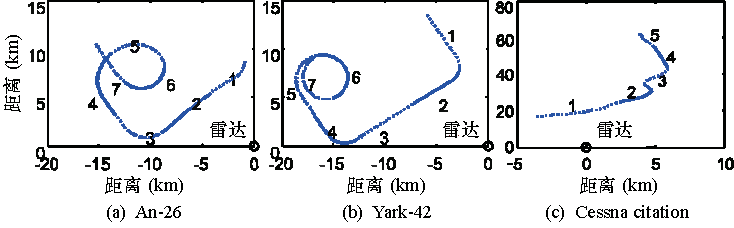
\includegraphics[width=0.8\linewidth]{figures/route.pdf}
\caption{实测数据集中三架目标飞机航迹在地面上的投影} 
\label{fig:route} 
\end{figure}

% --- 数据集示意图占位符 ---
\begin{figure}[h!]
    \centering
    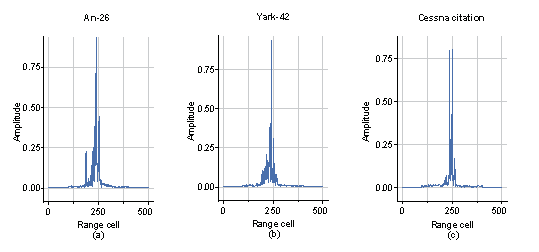
\includegraphics[width=0.75\linewidth]{figures/measured.pdf}
    \caption{实测数据集中3类飞机目标在1st方位角下的HRRP样本示例}
    \label{fig:dataset_chap3}
\end{figure}

实测数据上的识别准确率结果如表~\ref{tab:real_data_accuracy}~所示。首先,在性能更强的 服务器 平台上,SHARP ($\kappa=0.5$) 方法在实测数据上也展现出良好的性能,1-shot 和 5-shot 准确率分别达到了 58.31\% 和 71.05\%。将 SHARP ($\kappa=0.5$) 部署到树莓派后,其 1-shot 和 5-shot 准确率分别为 57.14\% 和 69.88\%。与 服务器 平台相比,准确率出现了轻微的下降(约 1.2\% 和 1.17\%),这可能源于模型转换过程中的精度损失、ONNX Runtime 实现与 PyTorch 的细微差异或 CPU 计算的数值稳定性问题。然而,这种程度的下降在可接受范围内,表明 SHARP 模型的核心识别能力在转换和部署后得到了有效保持。进一步地,我们在树莓派上比较了不同方法。SHARP ($\kappa=0.5$) 显著优于同样部署在树莓派上的 ProtoNet (1D-CNN),后者在 1-shot 和 5-shot 任务上分别仅获得 48.72\% 和 61.53\% 的准确率。这再次证明了利用 VLM 强大表征能力的优势,即使在资源受限的平台上,这种优势依然存在。同时,对比 SHARP ($\kappa=0.5$) 和 SHARP ($\kappa=0$) 在树莓派上的结果,可以看到语义精炼带来的提升是明显的,尤其是在样本极其稀疏的 1-shot 场景下,语义信息的校准作用更为关键。

\begin{table}[h!]
\centering
\caption{不同方法与平台在实测 HRRP 数据上的 3-way K-shot 识别准确率对比}
\label{tab:real_data_accuracy}
\resizebox{0.9\linewidth}{!}{%
\begin{tabular}{llcc}
\toprule
\textbf{部署平台} & \textbf{识别方法} & \makecell{\textbf{3-way 1-shot}\\\textbf{Acc. (\%)}} & \makecell{\textbf{3-way 5-shot}\\\textbf{Acc. (\%)}} \\
\midrule
服务器 (GPU) & SHARP ($\kappa=0.5$) & 58.31 $\pm$ 1.95 & 71.05 $\pm$ 1.28 \\
\midrule
Raspberry Pi 4B (CPU) & ProtoNet (1D-CNN) & 48.72 $\pm$ 2.10 & 61.53 $\pm$ 1.45 \\
Raspberry Pi 4B (CPU) & SHARP ($\kappa=0$) & 54.08 $\pm$ 2.01 & 67.55 $\pm$ 1.33 \\
\textbf{Raspberry Pi 4B (CPU)} & \textbf{SHARP ($\kappa=0.5$)} & \textbf{57.14 $\pm$ 1.98} & \textbf{69.88 $\pm$ 1.30} \\
\bottomrule
\end{tabular}%
} % End resizebox
\end{table}
\captionsetup{skip=5pt}

\begin{table}[h!]
\centering
\caption{不同方法与平台在实测 HRRP 数据上的平均单样本推理时延对比}
\label{tab:real_data_latency}
\resizebox{0.8\linewidth}{!}{%
\begin{tabular}{llc}
\toprule
\textbf{部署平台} & \textbf{识别方法} & \makecell{\textbf{Avg. 推理时延}\\\textbf{(ms per sample)}} \\
\midrule
服务器 (GPU) & SHARP ($\kappa=0.5$) & 18.7 \\
\midrule
Raspberry Pi 4B (CPU) & ProtoNet (1D-CNN) & 165.2 \\
Raspberry Pi 4B (CPU) & SHARP ($\kappa=0$) & 910.5 \\
\textbf{Raspberry Pi 4B (CPU)} & \textbf{SHARP ($\kappa=0.5$)} & \textbf{935.8} \\
\bottomrule
\end{tabular}%
} % End resizebox
\end{table}
\captionsetup{skip=5pt}

推理时延的对比结果呈现在表~\ref{tab:real_data_latency}~中。在 服务器 平台上利用 GPU 加速,SHARP ($\kappa=0.5$) 处理单个样本的平均时延仅为 18.7 ms,能够满足许多实时性要求较高的场景。然而,当转移到树莓派 4B 并仅使用 CPU 进行推理时,情况发生了显著变化。轻量级的 ProtoNet (1D-CNN) 在树莓派上的推理时延约为 165.2 ms,相对较快。相比之下,SHARP 方法由于需要通过适配器并将数据送入冻结的ViT-B/32 视觉编码器进行特征提取,其计算量远大于简单的 1D-CNN。SHARP ($\kappa=0$) 在树莓派上的平均推理时延达到了 910.5 ms,接近 1 秒。包含 SemAlign 模块的 SHARP ($\kappa=0.5$) 时延略有增加,达到 935.8 ms。这表明 SemAlign 模块带来的额外计算开销相对于 VLM 主干来说是比较小的(约 25.3 ms),但 VLM 本身的计算成本在没有 NPU 加速的 CPU 上是相当高的。

\section{本章小结}
\label{sec:semantic_summary}

本章针对小样本 HRRP 识别中特征判别力不足及语义信息利用困难的核心挑战,提出了一种基于跨模态语义嵌入的小样本HRRP元学习识别方法。该方法旨在有效利用大规模预训练VLM的强大表征能力,同时克服一维 HRRP 信号与 VLM 二维视觉输入之间的模态鸿沟,并缓解 VLM 可能存在的“语义偏见”问题。

所提SHARP首先通过语义进化和 VLM 文本编码器 $f_T$ 获取高质量的类别语义特征 $\mathbf{z}_T$。其次,设计一个轻量级的可训练 1D-to-2D 输入端适配器 $h_{1D2D}$,将 HRRP 信号 $\mathbf{x}_H$ 转换为伪图像 $\mathbf{x}_{pseudo}$。然后,利用 VLM 冻结的视觉编码器 $f_V$ 提取视觉特征 $\mathbf{z}_V$。关键创新在于适配器的协同训练目标,它联合优化了跨模态对齐损失 $L_{align}$和视觉特定对比损失 $L_{cl\_v2v}$。前者确保 $\mathbf{z}_V$ 与 $\mathbf{z}_T$ 对齐,迁移 VLM 的高级语义知识;后者强制 $\mathbf{z}_V$ 自身具有良好的类内聚合和类间分离特性,保留 HRRP 信号的内在结构信息。之后,通过预训练一个 SemAlign 模块 $h_F$,学习利用语义 $\mathbf{z}_T$ 来重建理想的视觉表示。最后,在元测试阶段,结合基础视觉原型 $\mathbf{u}_c$和语义精炼的重建原型 $\mathbf{r}_c$形成最终分类原型 $p_c$,并基于与查询特征 $\mathbf{z}_V$ 的相似度进行分类。

实验结果验证了SHARP相对于传统 FSL 方法和简单融合基线的显著优势。消融研究特别强调了协同训练目标中视觉对比损失 $L_{cl\_v2v}$ 对于提升特征判别性的关键作用,以及 SemAlign 模块带来的进一步性能增益。本章工作成功地将 VLM 的强大视觉能力适配到 HRRP 领域,并通过协同训练和多阶段语义利用策略,为解决小样本雷达信号识别问题提供了一种有效且高效的新范式。然而,实验结果也清晰地揭示了在嵌入式平台部署基于 ViT 的 SHARP所面临的严峻挑战,特别是在推理速度方面。近 1 秒的单样本处理时延对于需要高实时性的应用场景是难以接受的。这主要是由于树莓派 4B 缺乏 NPU 硬件加速单元,导致 VLM 庞大的计算量完全由通用 CPU 承担。因此,虽然本次实验成功验证了 SHARP 方法在嵌入式平台上的功能可行性和精度优势,但也指明了未来优化方向。为了在保持高精度的同时提高嵌入式部署的效率,可以探索量化、剪枝等模型压缩技术、采用更轻量级的 VLM 骨干网络、或者针对性地优化适配器结构以减少计算量。此外,选择Jetson 系列、或带 AI 加速模块的开发板等带有 NPU 的嵌入式硬件将是实现高性能部署的关键。总而言之,实测和硬件部署实验肯定了 SHARP 方法的有效性和潜力,同时也为后续的工程化落地提出了明确的性能优化需求。